\documentclass[10pt,twocolumn]{article}
\usepackage[margin=0.75in,columnsep=0.25in]{geometry}
\usepackage[T1]{fontenc}
\usepackage{times}
\usepackage{microtype}
\usepackage{graphicx}
\usepackage{booktabs}
\usepackage{amsmath}
\usepackage{tikz}
\usetikzlibrary{positioning,arrows.meta}
\usepackage[numbers,sort&compress]{natbib}
\usepackage[hidelinks]{hyperref}
\usepackage{titlesec}
\titlespacing*{\section}{0pt}{1.0ex plus 0.5ex}{0.6ex}
\titlespacing*{\subsection}{0pt}{0.8ex plus 0.3ex}{0.4ex}
\setlength{\abovecaptionskip}{4pt}
\setlength{\textfloatsep}{8pt plus 2pt}
\setlength{\dbltextfloatsep}{8pt plus 2pt}
\raggedbottom

\title{\vspace{-1.5em}\Large Where does GPT-2 small store sentiment?\\A layer-by-layer probing study with controls}
\author{Md Fajla Rabby}
\date{\vspace{-2em}}

\begin{document}
\maketitle

\begin{abstract}
A language model like GPT-2 turns each word of a sentence into a list of numbers and updates that list as it passes through the model's 12 internal blocks. I asked a simple question: after which block can a plain linear classifier tell from these numbers whether a movie review is positive or negative? I trained one classifier, called a probe, at each of 13 points in GPT-2 small, using sentences from the SST-2 dataset. To check that the answer reflects what GPT-2 learned, I compared every probe with four baselines, including a word-counting classifier and an untrained copy of GPT-2, repeated everything five times, and tested differences statistically. Sentiment can be read after the first block (67.2\% accuracy) and is clearest after blocks 7 to 9 (84 to 85\%). The probe beats word counting from block 5 on and beats the untrained model by up to 30 points. A small negation test shows the same split: early blocks treat \textit{not} as a negative word, while from block 7 \textit{not good} reads as negative and \textit{not bad} reads as less negative.
\end{abstract}

\section{Introduction}

Large language models are trained only to predict the next word, yet they end up tracking things like topic, grammar and tone. One way to look for this is a probe: a small, simple classifier trained on the model's internal numbers. If a probe can predict some property from the numbers at a certain depth, the property is readable there.

A good probe score is easy to over-read. The probe might learn the task from its own training data, an untrained network of the same shape might give useful numbers too, and the test sentences might differ from the training sentences in some way that moves the score. So a probe result only means something next to the right comparisons.

I studied one property, sentiment, in one model, GPT-2 small \citep{radford2019language}, and asked two questions. At which depth does sentiment become readable from the last word of a sentence? And how much of it goes beyond what simple word counting already gets?

The study adds three things: a depth-by-depth accuracy curve checked against four baselines over five repeated runs; a check that differences between the training and test sentences do not inflate the results; and a negation test that separates GPT-2's later blocks from any word-counting model. It runs on an ordinary laptop CPU in about an hour.

\section{Method}

\begin{figure*}[t]
\centering
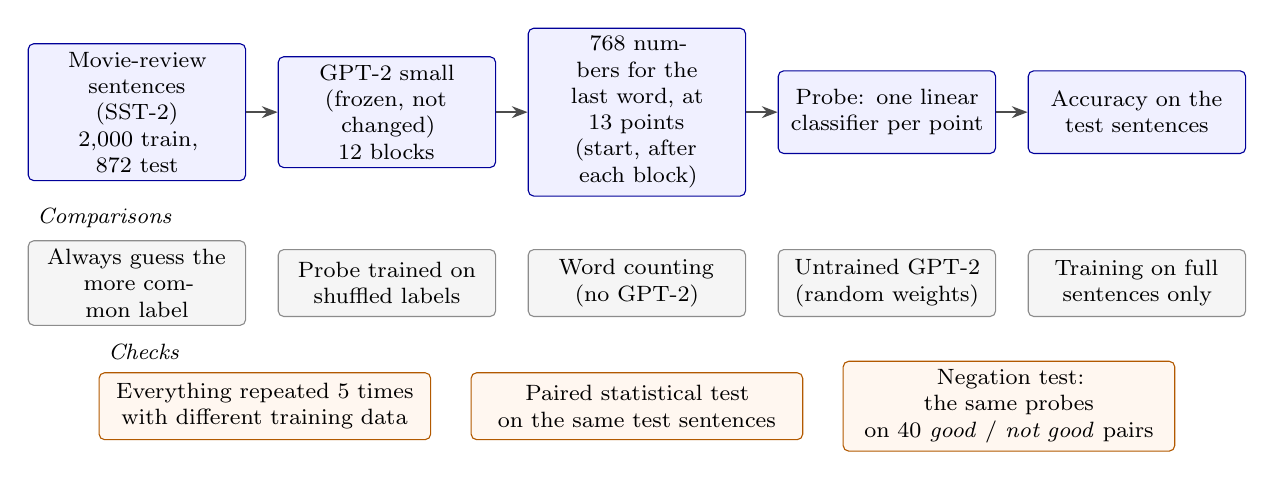
\begin{tikzpicture}[
  node distance=0.45cm and 0.4cm,
  box/.style={draw=blue!60!black, fill=blue!6, rounded corners=2pt, align=center, font=\footnotesize, minimum height=1.05cm, text width=2.55cm, inner sep=3pt},
  ctrl/.style={draw=black!45, fill=black!4, rounded corners=2pt, align=center, font=\footnotesize, minimum height=0.85cm, text width=2.55cm, inner sep=3pt},
  eval/.style={draw=orange!70!black, fill=orange!6, rounded corners=2pt, align=center, font=\footnotesize, minimum height=0.85cm, text width=4.0cm, inner sep=3pt},
  arr/.style={-{Stealth[length=2mm]}, thick, black!70}
]
\node[box] (data) {Movie-review sentences\\(SST-2)\\2,000 train, 872 test};
\node[box, right=of data] (model) {GPT-2 small\\(frozen, not changed)\\12 blocks};
\node[box, right=of model] (feat) {768 numbers for the\\last word, at 13 points\\(start, after each block)};
\node[box, right=of feat] (probe) {Probe: one linear\\classifier per point};
\node[box, right=of probe] (acc) {Accuracy on the\\test sentences};
\draw[arr] (data) -- (model);
\draw[arr] (model) -- (feat);
\draw[arr] (feat) -- (probe);
\draw[arr] (probe) -- (acc);

\node[ctrl, below=0.75cm of data] (c1) {Always guess the\\more common label};
\node[ctrl, right=of c1] (c2) {Probe trained on\\shuffled labels};
\node[ctrl, right=of c2] (c3) {Word counting\\(no GPT-2)};
\node[ctrl, right=of c3] (c4) {Untrained GPT-2\\(random weights)};
\node[ctrl, right=of c4] (c5) {Training on full\\sentences only};
\node[font=\footnotesize\itshape, anchor=south west] at ([yshift=1pt]c1.north west) {Comparisons};

\node[eval, below=0.7cm of c3] (e2) {Paired statistical test\\on the same test sentences};
\node[eval, left=0.5cm of e2] (e1) {Everything repeated 5 times\\with different training data};
\node[eval, right=0.5cm of e2] (e3) {Negation test: the same probes\\on 40 \textit{good} / \textit{not good} pairs};
\node[font=\footnotesize\itshape, anchor=south west] at ([yshift=1pt]e1.north west) {Checks};
\end{tikzpicture}
\caption{Study design. Top: the main measurement. Middle: the comparisons each probe is judged against. Bottom: how the results were checked.}
\label{fig:pipeline}
\end{figure*}

Figure~\ref{fig:pipeline} shows the whole design.

\subsection{What is measured}
GPT-2 small reads a sentence one word piece at a time. Each piece is represented by 768 numbers, and each of the model's 12 blocks adds to those numbers as the sentence is processed. I recorded the numbers for the last word of each sentence at 13 points: at the start, before any block (point 0), and after each block (points 1 to 12). In GPT-2 a word can only use information from the words before it, so the last word is the only position that has seen the whole sentence. The model was loaded with the TransformerLens library \citep{nanda2022transformerlens} and was never changed.

\subsection{Data}
SST-2 is a set of short movie-review sentences labelled positive or negative \citep{socher-etal-2013-recursive}. Its 872 validation sentences (444 positive, 428 negative) are my test set; the official test labels are not public. The training part also contains many short phrases, so I kept only examples with at least six words, removed duplicates and removed anything that also appears in the test set. Each run trained on 1,000 positive and 1,000 negative examples, and the five runs used five separate samples with no overlap.

The training and test sentences differ in one visible way: 94\% of test sentences end with a full stop, but only 29\% of training examples do. Section~\ref{sec:mismatch} tests whether this matters.

\subsection{The probe}
At each point the probe is a logistic regression, a classifier that draws one straight dividing line (a flat boundary, in 768 dimensions) between positive and negative sentences. Before training, each of the 768 numbers is rescaled using the training sentences only, because their size grows about 90-fold from point 0 to point 12. The amount of regularisation, a setting that stops the probe from memorising its training data, was chosen by cross-validation on the training sentences, so the test sentences were used only once, for the final score.

\subsection{Comparisons}
Each probe was judged against four baselines. Always guessing the more common label gives 50.9\%. A probe trained on randomly shuffled labels checks that no test information leaks into training. A word-counting classifier, often called bag of words, uses only which words a sentence contains, with no GPT-2 at all. An untrained GPT-2, with the same structure but random weights, shows how much the architecture alone gives.

\subsection{Repeats and statistics}
The whole experiment was run five times, each with its own training sample and random seeds, on the same test set. Figures show the mean and spread over the five runs. To compare two settings, I used a paired bootstrap: the 872 test sentences are resampled 10,000 times, and each time I check which setting got more of the same sentences right. This gives a 95\% range for the difference. The comparisons were decided before I looked at their results, and I used a strict cutoff ($p < 0.0042$) because twelve were made.

\subsection{Negation test}
I built 40 sentence pairs from one template, such as \textit{the plot was good .} and \textit{the plot was not good .}, using five subjects, four positive words (\textit{good}, \textit{great}, \textit{funny}, \textit{charming}) and four negative ones (\textit{bad}, \textit{boring}, \textit{dull}, \textit{awful}). The trained probes were applied as they were, with no retraining, and I measured how much adding \textit{not} moved each probe's score. The \emph{negation interaction} is how much more \textit{not} raises the score for negative words than for positive words. A word-counting model treats \textit{not} as a word with one fixed score, so for it this number is always exactly zero.

\section{Results}

\begin{figure}[t]
\centering
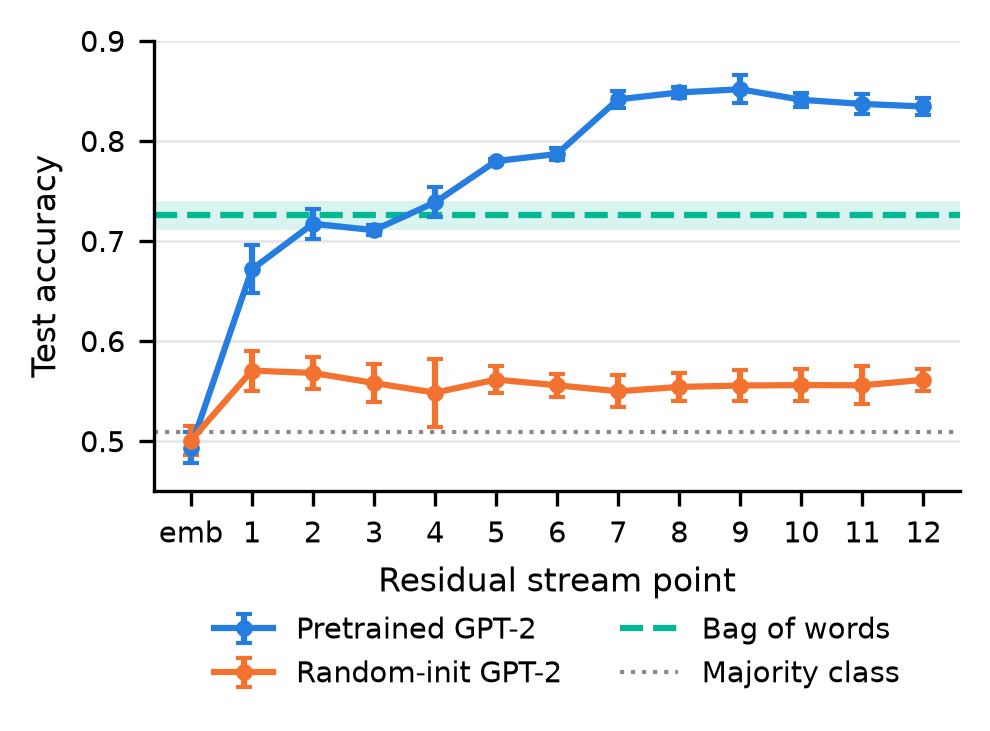
\includegraphics[width=\columnwidth]{figures/paper_fig1}
\caption{Probe accuracy on the 872 test sentences at each point (emb = before any block; 1 to 12 = after that block). Dots and bars show the mean and standard deviation over five runs. The green band is the word-counting classifier's mean $\pm$ one standard deviation.}
\label{fig:layers}
\end{figure}

\begin{table}[t]
\centering
\small
\resizebox{\columnwidth}{!}{\begin{tabular}{lrrr}
\toprule
Comparison & Diff. (pp) & 95\% interval (pp) & $p$ \\
\midrule
Block 9 vs block 7 & +1.0 & [-0.3, +2.3] & 0.119 \\
Block 9 vs block 12 & +1.7 & [+0.7, +2.8] & 0.001 \\
Block 1 vs word counting & -5.4 & [-7.8, -3.0] & $<$0.001 \\
Block 4 vs word counting & +1.3 & [-1.3, +3.8] & 0.305 \\
Block 5 vs word counting & +5.4 & [+3.0, +7.9] & $<$0.001 \\
Block 7 vs word counting & +11.6 & [+9.2, +14.0] & $<$0.001 \\
Block 1, trained vs untrained & +10.1 & [+7.7, +12.5] & $<$0.001 \\
Block 9, trained vs untrained & +29.6 & [+27.0, +32.2] & $<$0.001 \\
\bottomrule
\end{tabular}}
\caption{Paired comparisons on the test sentences. Differences and 95\% ranges are in percentage points (pp), averaged over five runs. A $p$ below 0.0042 counts as a clear difference.}
\label{tab:comparisons}
\end{table}

\subsection{Sentiment across the model}
Figure~\ref{fig:layers} shows the main result. Before any block the probe is at chance (49.4\%). That is expected: almost every test sentence ends with the same full stop, so at point 0 the last word carries no information about the rest of the sentence. After one block, accuracy is 67.2\%. It keeps rising and reaches 84.2\% after block 7, 84.8\% after block 8 and 85.2\% after block 9.

There is no single best block. The best point changed from run to run (7, 8, 8, 9 and 11), and block 9 cannot be told apart from block 7 (Table~\ref{tab:comparisons}). The last two blocks are a little worse: block 12 is 1.7 points below block 9 and block 11 is 1.5 points below, and both differences pass the strict cutoff. Results were stable across runs, with standard deviations of 0.3 to 2.4 points.

\subsection{Against the baselines}
The probe trained on shuffled labels stayed between 47.1\% and 53.7\% at every point (checked in the first run), so nothing leaked from the test set. Word counting reached 72.5\%. After one block GPT-2 is 5.4 points worse than word counting, after block 4 the two are level, and from block 5 on GPT-2 is clearly better: by 5.4 points after block 5 and 11.6 points after block 7. The early blocks hold about as much sentiment as a word count does. The extra comes in the middle of the model.

The untrained GPT-2 scored between 54.8\% and 57.0\% at every point after the start, with no rise across the model. It is slightly above chance because even random weights keep different words apart and mix them together. The trained model was 10.1 points better after block 1 and 29.6 points better after block 9. The rising curve comes from what GPT-2 learned during training.

\subsection{Do the training sentences matter?}
\label{sec:mismatch}
Training examples were mostly phrases, while test sentences were full sentences ending in a full stop. To check the effect, I trained probes only on training examples that end in a full stop (about 570 per run) and compared them with random training sets of the same size. The full-stop probes were better at all four points tested (after blocks 1, 4, 7 and 9), by 2.3 to 4.8 points, and with less than a third of the data they matched the main 2,000-example probe (84.8\% against 85.2\% after block 9). The mismatch therefore pushes the main results slightly down rather than up. This check cannot tell whether the full stop itself or the use of complete sentences is what helps.

\begin{figure}[t]
\centering
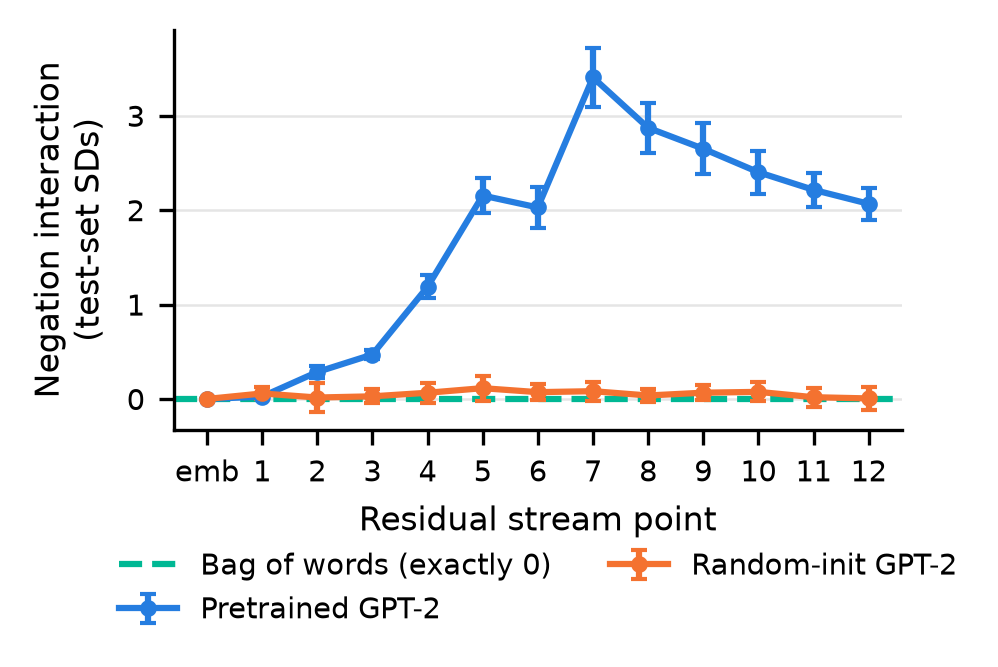
\includegraphics[width=\columnwidth]{figures/paper_fig2}
\caption{Negation interaction at each point: how much more adding \textit{not} raises the probe score for negative words than for positive words, measured in units of the score's spread on the test set. 40 sentence pairs; bars show the spread over five runs. Word counting always gives exactly 0.}
\label{fig:negation}
\end{figure}

\subsection{Negation}
After blocks 3 to 7, the probes label the plain template sentences correctly 91.5\% to 96.5\% of the time, so their scores on these short sentences are meaningful. Adding \textit{not} to a positive word lowers the score at every point after the start and flips the prediction to negative in 92\% of pairs after block 5 and 91\% after block 7.

Negative words behave differently. After blocks 1 to 4, adding \textit{not} to \textit{bad} or \textit{boring} also lowers the score, which is exactly what word counting does: in all five runs it learned a negative score for \textit{not} and applied it to every sentence. The effect is zero after blocks 5 and 6 and turns positive after block 7. The score rarely crosses to positive (at most 31\% of pairs), which matches how people read \textit{not bad}: less negative, but not quite positive.

Figure~\ref{fig:negation} puts this into one number per point. The interaction is near zero after block 1, grows through the middle blocks, peaks after block 7 and falls slightly towards the end. The untrained model stays near zero throughout. The change for \textit{not bad} happens between blocks 6 and 7, the same place where sentiment accuracy jumps from 78.7\% to 84.2\%. The two measurements line up, but this study does not show that one causes the other.

\section{Limitations}
A probe shows that information can be read from the model's numbers. It does not show that GPT-2 uses that information when it predicts the next word; that would need experiments that change the numbers and watch the output. The study covers one small model, one dataset of movie reviews and only the last word of each sentence. Five runs give a rough idea of the spread, and the test set was the same every time. The trained and untrained models were loaded with slightly different settings (the trained one with re-centred weights), which I do not expect to explain gaps of 10 to 30 points. The negation test uses one sentence template and 40 short pairs, and its interaction measure was defined after the results came in, although it follows directly from how word counting works.

\paragraph{Code and AI use.} The code, saved results and a full research log are in the project repository. An AI assistant (Claude, by Anthropic) helped write the code and draft this paper. I ran all the experiments and checked every number in the paper against the saved results.

{\small
\bibliographystyle{plainnat}
\bibliography{references}
}

\end{document}
